% Para compilar, use:
% pdflatex -shell-escape melissa_kthxbai.tex
%%%%%%%%%%%%%%%%%%%%%%%%%%%%%%%%%%%%%%%%%%%%%%%%%%%%%%%%%%%%%%%%%%%%%%%%%%%%%%%%%%%%%%%%%
% PREAMBULO
%%%%%%%%%%%%%%%%%%%%%%%%%%%%%%%%%%%%%%%%%%%%%%%%%%%%%%%%%%%%%%%%%%%%%%%%%%%%%%%%%%%%%%%%%
\documentclass{beamer}
% Temas do beamer
\usetheme{Boadilla}
%\usecolortheme{purple}
\usefonttheme[onlysmall]{structurebold}
\usenavigationsymbolstemplate{}
%\useoutertheme{smoothbars}
% This Charming Man palette from colorlovers.com
\definecolor{purple}{rgb}{0.5,0,0.5}
% Escolhendo as cores padrão do beamer
%\setbeamercolor{normal text}{fg=winterbland}
\setbeamercolor{structure}{fg=purple}
%\setbeamercolor{block title}{fg=lazereyes}
%\setbeamercolor{block body}{}
\setbeamercolor{alerted text}{fg=purple}
\setbeamercolor{frametitle}{fg=purple}
%
% Pacotes adicionais
\usepackage[utf8]{inputenc} % Para permitir a exibição correta de acentos
\usepackage[portuguese]{babel} % Para exibir palavras-chave em português
\usepackage{txfonts} % Fontes bonitas :)
\usepackage{colortbl}
\usepackage{eso-pic}
\usepackage{tikz}
\usetikzlibrary{positioning, arrows, shapes}
\usetikzlibrary{shapes}
% Define box and box title style
\tikzstyle{mybox} = [draw, very thick, rectangle, inner sep=10pt, inner ysep=20pt, fill=black, text=white, minimum width=\textwidth, minimum height=2cm]

\tikzstyle{redRectangle} = [
    rectangle,
    draw,
    fill=red!20,
    node distance=0.85 cm,
    text width=7 em,
    text centered,
    rounded corners,
    minimum height=4 em,
    minimum width=3 cm,
    thick
    ]
    \tikzstyle{blueRectangle} = [
    rectangle,
    draw,
    fill=blue!20,
    node distance=1.5 cm,
    text width=7 em,
    text centered,
    rounded corners,
    minimum height=4 em,
    minimum width=3 cm,
    thick
    ]
    \tikzstyle{yellowRectangle} = [
    rectangle,
    draw,
    fill=yellow!20,
    node distance=1.5 cm,
    text width=7 em,
    text centered,
    rounded corners,
    minimum height=4 em,
    minimum width=3 cm,
    thick
]
\tikzstyle{empty} = []
% Variáveis da apresentação
\title{Produzindo lindos relatórios com Pweave}
\author{Melissa Weber Mendonça}
\date{pythonbrasil[12]}
\logo{
\includegraphics[height=1.5cm]{brasao_UFSC.png}}
%%%%%%%%%%%%%%%%%%%%%%%%%%%%%%%%%%%%%%%%%%%%%%%%%%%%%%%%%%%%%%%%%%%%%%%%%%%%%%%%%%%%%%%%% 
% FIM DO PREAMBULO
%%%%%%%%%%%%%%%%%%%%%%%%%%%%%%%%%%%%%%%%%%%%%%%%%%%%%%%%%%%%%%%%%%%%%%%%%%%%%%%%%%%%%%%%%

\begin{document}

{% Definindo frame de título.
\setbeamertemplate{footline}{} 
\setbeamertemplate{headline}{}
% \usebackgroundtemplate{\includegraphics[width=\paperwidth,height=\paperheight]{imagens/linus.jpg}}%
\begin{frame}%

   \titlepage%
   
 \end{frame}%
}

\begin{frame}
  \frametitle{Motivação}
  \begin{center}
    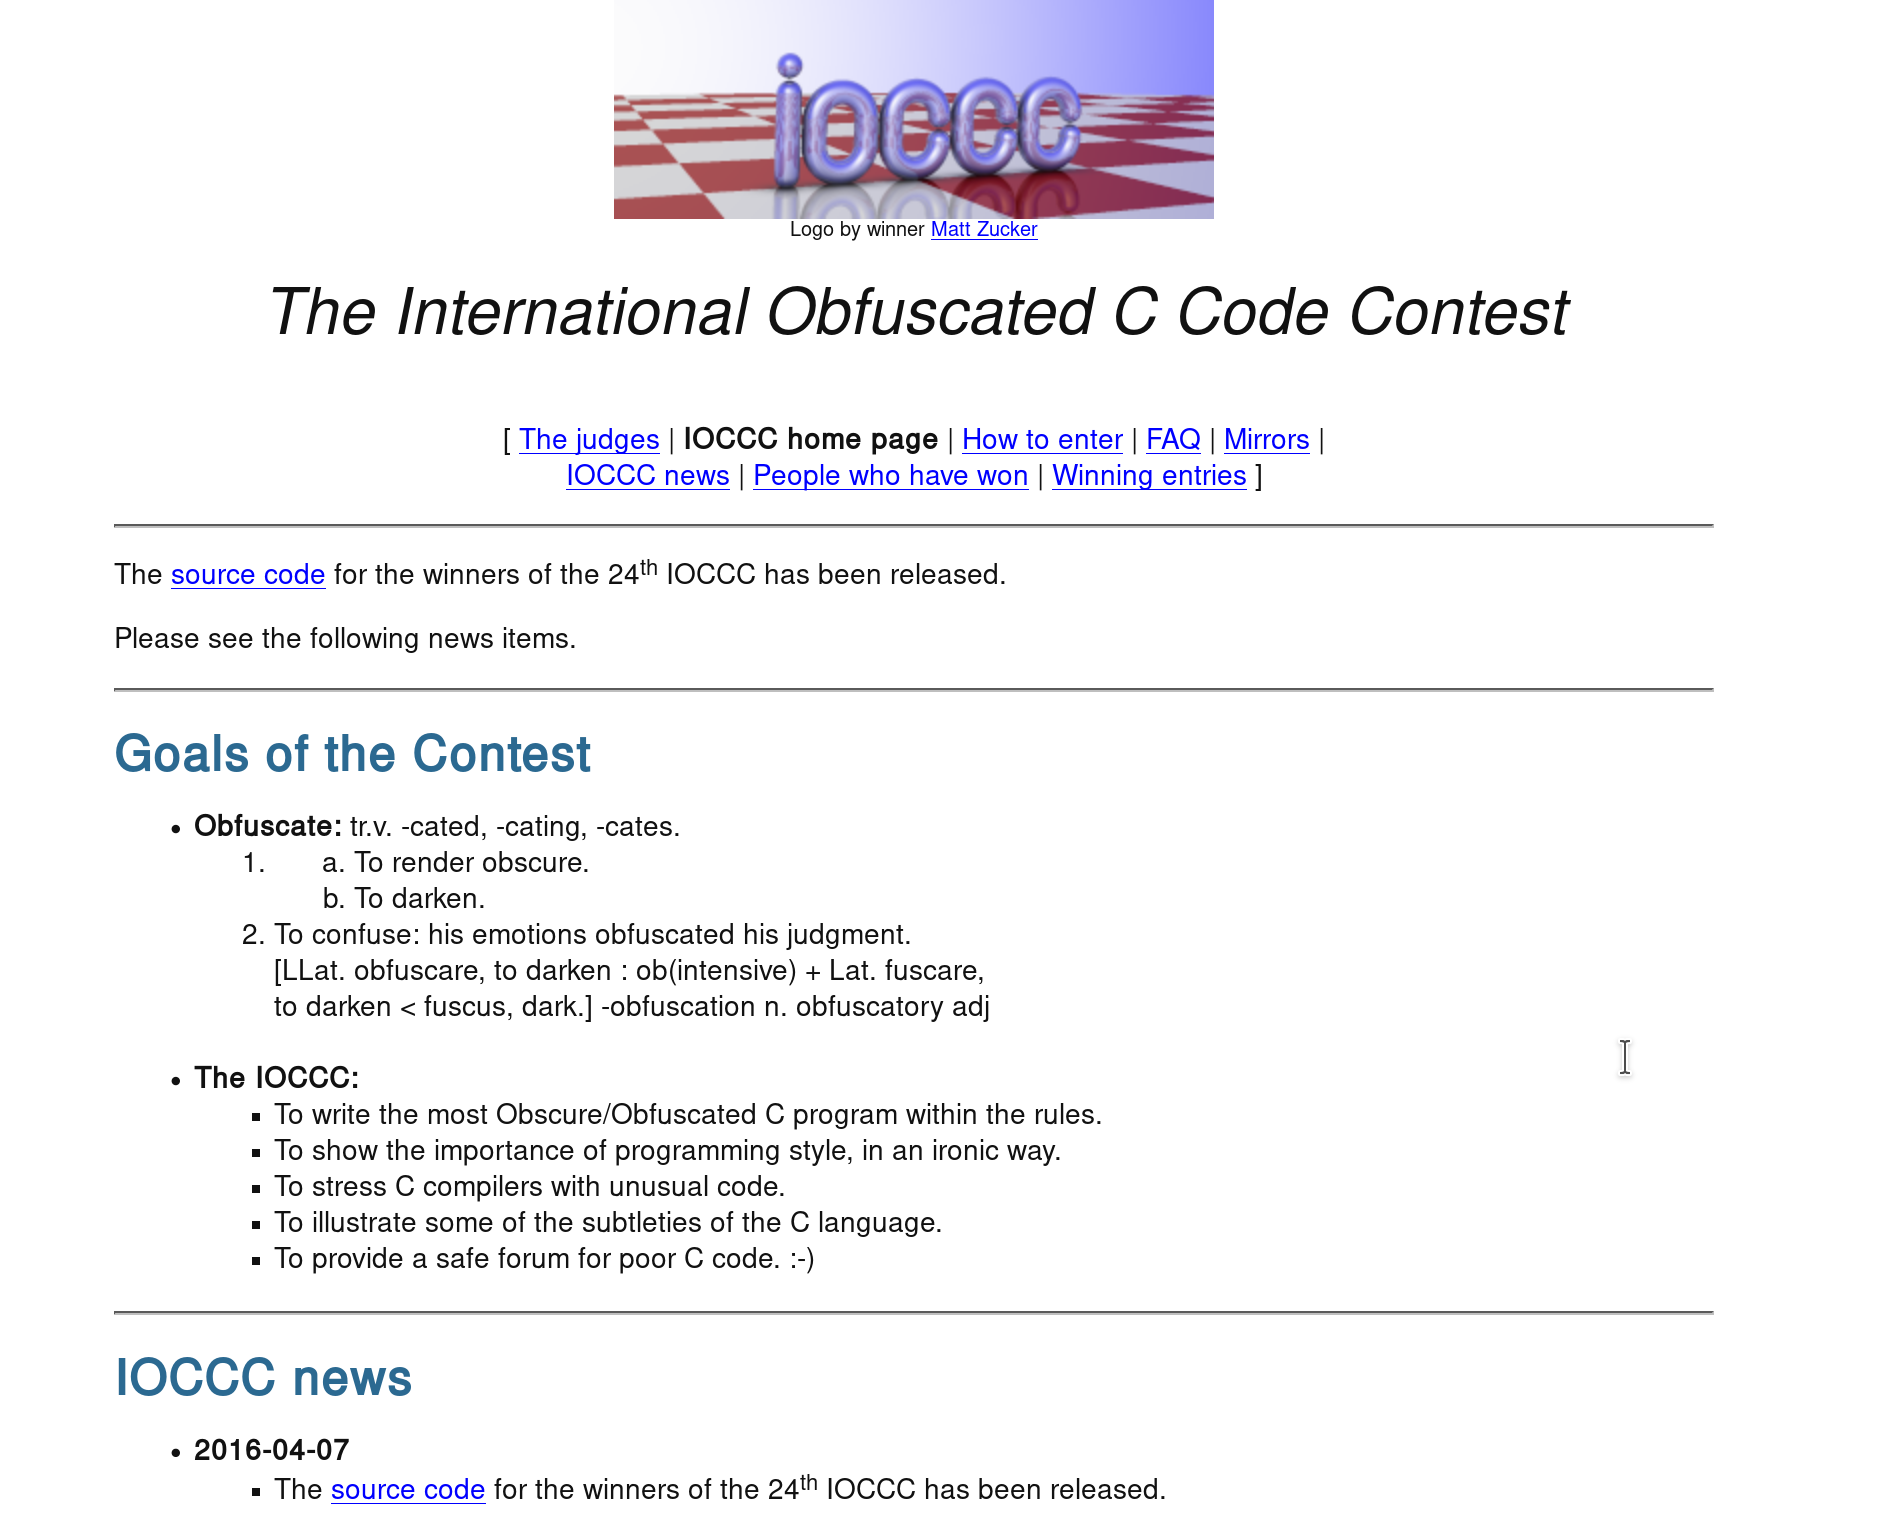
\includegraphics[width=0.9\textwidth]{obfuscated.png}
  \end{center}
\end{frame}

\begin{frame}
  \frametitle{Literate Programming}
  \begin{itemize}
  \item Linguagem natural + macros/código
  \item \emph{Compilável}
  \item Lógica da máquina v. Lógica humana
  \end{itemize}
  \begin{columns}
    \column{5cm}
    \begin{center}
      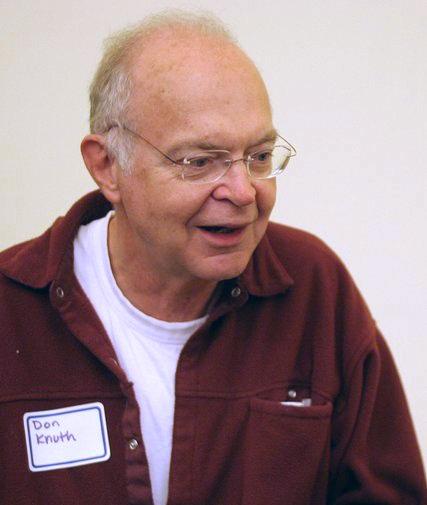
\includegraphics[width=3.4cm]{knuth.jpg}\\
      Don Knuth (1981)
    \end{center}
    \column{5cm}
    \begin{center}
      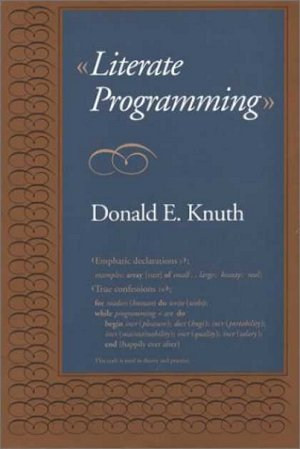
\includegraphics[width=3cm]{Literate_Programming_book_cover.jpg}
    \end{center}
  \end{columns}
\end{frame}

\begin{frame}
  \frametitle{Linguagem natural v. Linguagem de máquina}
%     Instead of imagining that our main task is to instruct a computer what to do, let us concentrate rather on explaining to human beings what we want a computer to do.
  % Overall, web is combination of two languages: 1) Document formatting Language 2) Programming language. Although Pascal and TeX is the most commonly used combination for Literate programming, documentation language may include TeX, Scribe, Troff while programming languages can be Pascal, A, ALGOL, LISP, COBOL, FORTRAN, APL, C, etc.[1]
  \begin{itemize}
  \item Código como literatura
  \item Descrever a lógica explicitamente
  \item Documentação orgânica
  \item \alert{Pesquisa e reproducibilidade}
  \end{itemize}
\end{frame}

\begin{frame}[fragile]
  \frametitle{Literate Programming: WEB}
  \begin{center}
    \begin{tikzpicture}
      \node[redRectangle] at (0,0) (source) {``Literate source file''};
      \draw[very thick] (source.east) -- (4.6,0);
      \node[] at (3,0.2) {Preprocessador};
      \draw[very thick, ->] (4.6,0) -- (5.3,1);
      \draw[very thick, ->] (4.6,0) -- (5.3,-1);
      \node[yellowRectangle] at (6,1.8) {``tangled'' (compilável)};
      \node[blueRectangle] at (6,-1.8) {``woven'' (documentação)};
    \end{tikzpicture}
  \end{center}

  \begin{center}
    \href{https://github.com/zyedidia/Literate/blob/master/examples/wc.lit}{\beamergotobutton{wc.lit}}
  \end{center}
\end{frame}

\begin{frame}
  \frametitle{Implementações}
  \begin{itemize}
  \item WEB \textemdash\ Pascal + \TeX\ (Knuth) 
  \item CWEB \textemdash\ C + \TeX\ (Knuth e Silvio Levy)
  \item Sweave \textemdash\ R + \TeX
  \item knitr \textemdash\ R+\TeX
  \item noweb \textemdash\ Linguagem? + Formato? (HTML)
  \item iJulia
  \item iPython/Notebooks
  \item \alert{Pweave} \textemdash\ Python + Formato?
  \end{itemize}
\end{frame}

\begin{frame}
  \frametitle{O que não é Literate Programming}
  \begin{itemize}
  \item Código bem documentado
  \item Relatórios incluindo código e texto 
  \item Documentação automática
  \item Notebooks escritos de maneira tradicional
  \end{itemize}
\end{frame}

\begin{frame}
  \frametitle{}
  \begin{center}
    \begin{block}
      {Donald Knuth. "Literate Programming (1984)" in Literate Programming. CSLI, 1992, pg. 99.}
      Let us change our traditional attitude to the construction of programs: Instead of imagining that our main task is to instruct a computer what to do, let us concentrate rather on explaining to human beings what we want a computer to do.
      
      The practitioner of literate programming can be regarded as an essayist, whose main concern is with exposition and excellence of style. Such an author, with thesaurus in hand, chooses the names of variables carefully and explains what each variable means.
    \end{block}
  \end{center}
\end{frame}

\begin{frame}
  \frametitle{Pweave}
  \begin{center}
    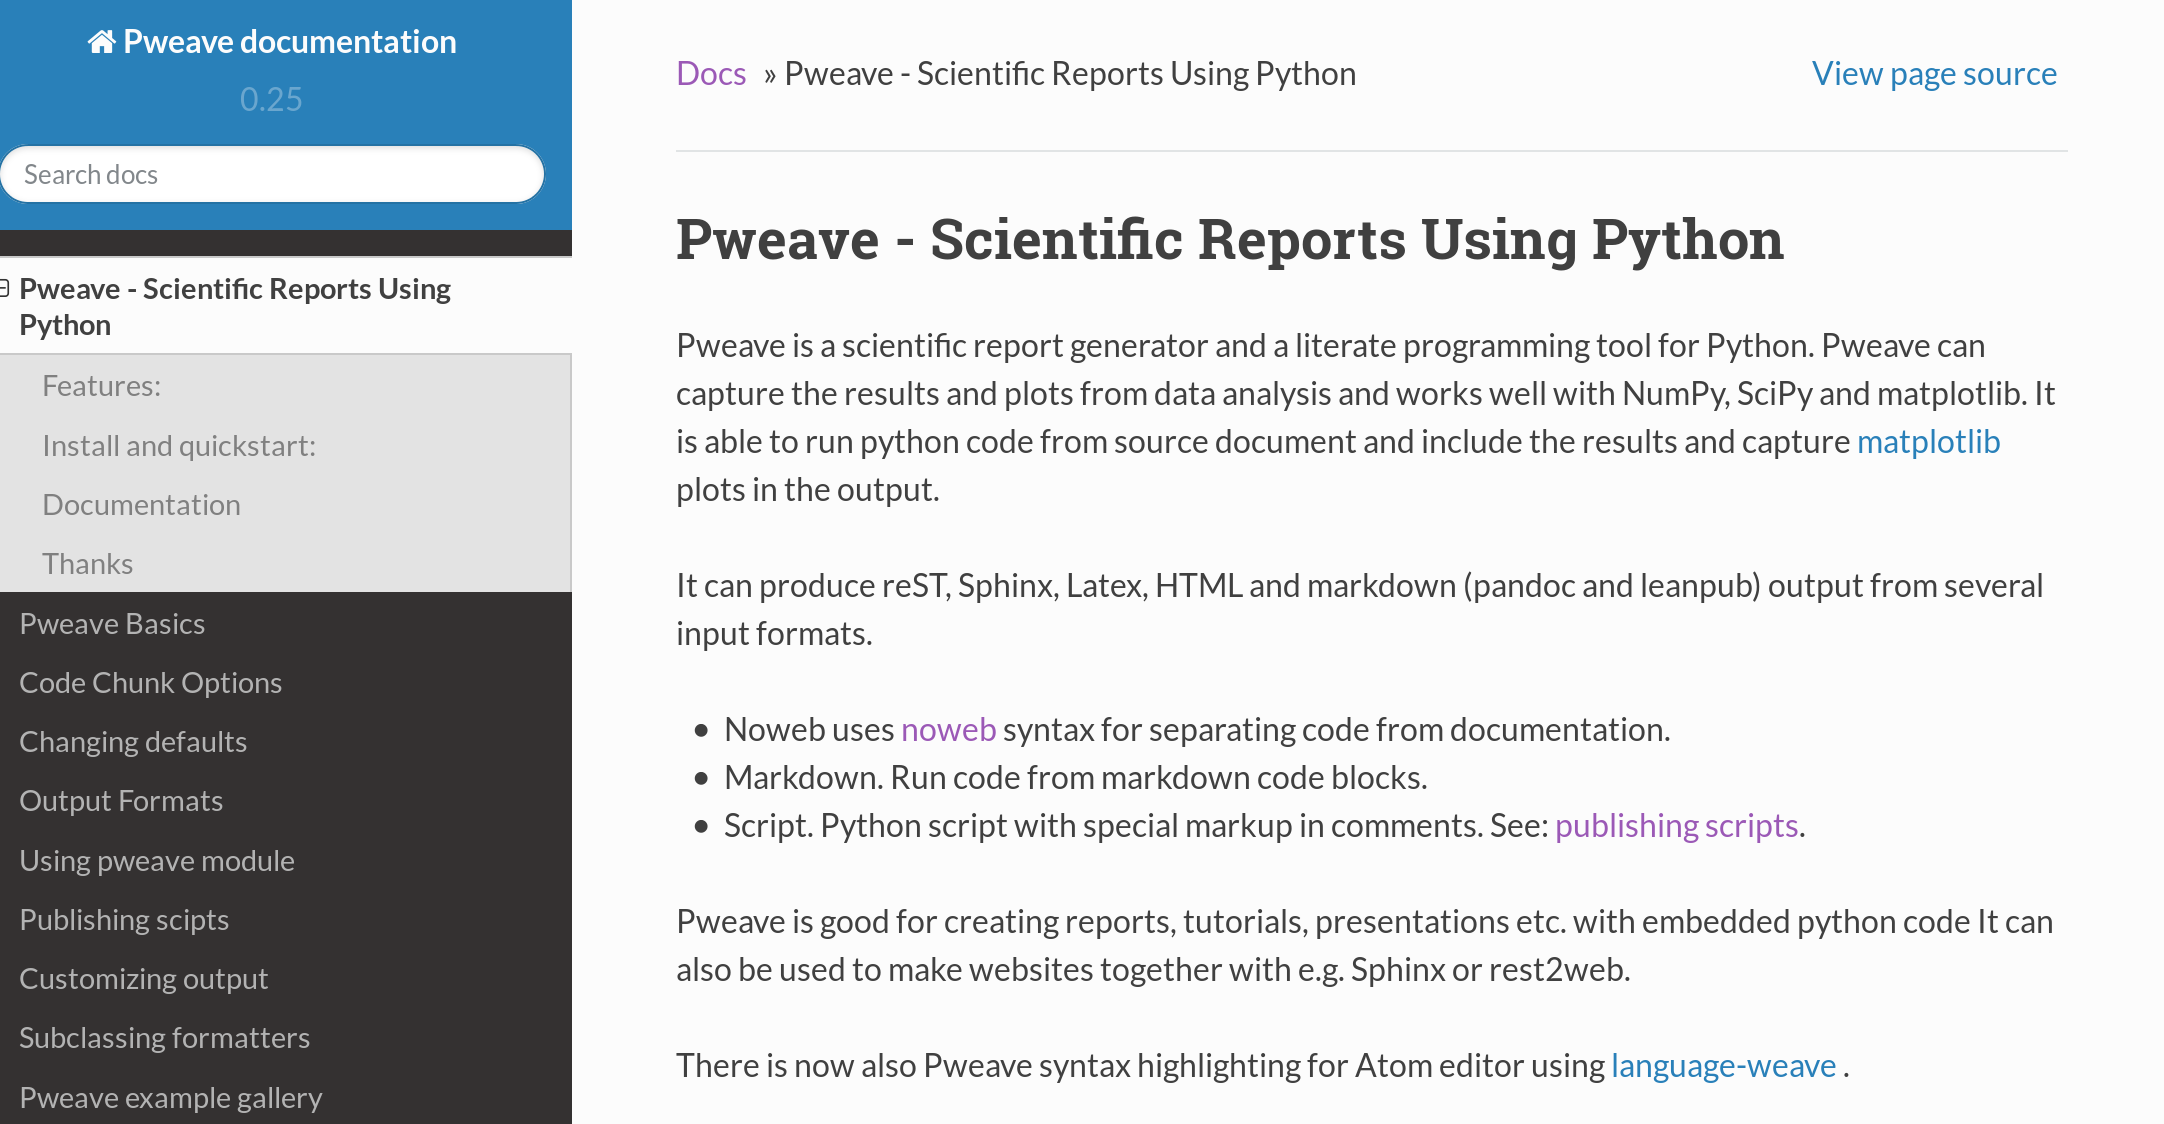
\includegraphics[width=\textwidth]{pweave.png}
  \end{center}
\end{frame}

\begin{frame}[fragile]
  \frametitle{Pweave}
  \begin{itemize}
  \item input: documentação e código separados por markup \href{exemplos/ctd.py}{\beamergotobutton{exemplo}}
  \end{itemize}      

  \vfill
  
  Para gerar um HTML simples:
  \begin{center}
    \begin{tikzpicture}
      \node[mybox] (box) {
        \begin{minipage}{0.8\textwidth}
          \texttt{\$ pypublish [-t bootstrap/cerulean] ctd.py}
        \end{minipage}
      };
      % \node[draw, fill=white, text=black, right=10pt, rounded corners] at (box.north west) {
      % \textbf{#2}
      % };
    \end{tikzpicture}
  \end{center}
  Para gerar um PDF:
  \begin{center}
    \begin{tikzpicture}
      \node[mybox] (box) {
        \begin{minipage}{0.8\textwidth}
          \texttt{\$ pypublish -f pdf ctd.py}
        \end{minipage}
      };
      % \node[draw, fill=white, text=black, right=10pt, rounded corners] at (box.north west) {
      % \textbf{#2}
      % };
    \end{tikzpicture}
  \end{center}
\end{frame}

\begin{frame}[fragile]
  \frametitle{Code chunks em documentos: \texttt{noweb}}
  Dentro de algum documento \texttt{.(ext)\alert{w}}:
  \begin{center}
    \begin{tikzpicture}
      \node[rectangle, rounded corners, very thick, draw] {%
        \parbox{8cm} e \texttt{\%>} ou \texttt{<\%=} e \texttt{\%>} (imprime o resultado)
  \end{itemize}
\end{frame}  

% Pweave currently has the following options for processing the code chunks.
% name, label
%     If the first option of chunk is unnamed it will become the chunk name, you can also set the chunk name using the name or label (for Sweave compatibility) keys. All of these definitions are equal <<analysis, Fig = True>>=, <<Fig = True, name = 'analysis'>>=, <<Fig = True, label = 'analysis'>>=. Chunk names are used for figure names, but expanding named chunks in the Pweave todo list.
% echo = True or (False)
%     Echo the python code in the output document. If False the source code will be hidden.
% evaluate = True or (False).
%     Evaluate the code chunk. If False the chunk won’t be executed.
% results = 'verbatim'
%     The output format of the printed results. ‘verbatim’ for literal block, ‘hidden’ for hidden results or anything other string for raw output (I tend to use ‘tex’ for Latex and ‘rst’ for rest. Raw output is useful if you wan’t to e.g. create tables from code chunks.
% term = False or (True)
%     If True the output emulates a terminal session i.e. the code chunk and the output will be printed as a doctest block. Can also be used in latex documents, where the output will formatted as verbatim.
% include = True or (False)
%     If include is True generated figures are automatically included in the document otherwise figures are generated, but not included. This is useful if you want more control over figure formatting e.g. use subfigures in Latex.
% fig = True or (False)
%     Whether a matplotlib plot produced by the code chunk should be included in the file. The figure will be added with ‘.. image::’ directive in .rst and \includegraphics tag in .tex documents. See the ‘caption’ option if you want to use figure environment. As of version 0.21 Pweave supports multiple figures per code chunk.
% caption = ''
%     A string providing a caption for the figure produced in the code chunk. Can only be used with ‘fig = True’ option.
% width
%     The width of the created figure in the document (using format specific markup e.g. “12cm”, “600px”, “linewidth”). The default width depends on the output format.
% f_size = (8,6)
%     Saved matplotlib figure size in inches a tuple (w, h).
% f_spines = True
%     Removes spines from matplotlib figures right and top if False.
% f_env
%     Add environment that goes around figures in LaTex output e.g. sidefigure
% f_pos = "htpb"
%     Sets the figure position for latex figures.
% wrap = True or (False,"code", "results")
%     Controls wrapping of long lines. If True both code and output are wrapped to 75 characters. You can also specify “code” or “results” options to wrap only input or output.
% complete = True
%     Used to include code spanning multiple chunks before it get executed. Useful for e.g. documenting class definitions. Use complete = False all but the last chunk and set the last one as complete = True. Pweave executes all of the chunks together and includes the results after the last one. See: Splitting code to multiple chunks example.
% source
%     Read chunk contents from file or python module or file. e.g. source = “mychunk.py”
% engine
%     Choose engine running the code. “python” or “shell”. If “shell” code will be run line by line using subprocess.Open

\begin{frame}
  \frametitle{Formatos de saída}
  \begin{itemize}
  \item HTML com pygments
  \item markdown
  \item pandoc/pandoc2html/pandoc2latex
  \item tex/texminted/texpygments
  \item texpweave
  \item rst
  \item sphinx
  \item leanpub
  \end{itemize}
\end{frame}

\begin{frame}[fragile]
  \frametitle{Em ação}
  \href{exemplos/exemplo.texw}{Exemplo \LaTeX: \beamergotobutton{exemplo}}

  \begin{center}
    \begin{tikzpicture}
      \node[mybox] (box) {
        \begin{minipage}{0.8\textwidth}
          \texttt{\$ pweave -f tex exemplo.texw}\\
          \texttt{\$ pdflatex exemplo.tex}
        \end{minipage}
      };
    \end{tikzpicture}
  \end{center}
\end{frame}

\begin{frame}[fragile]
  \frametitle{Em ação}
  \href{exemplos/fird.mdw}{Exemplo markdown: \beamergotobutton{exemplo}}

  \begin{center}
    \begin{tikzpicture}
      \node[mybox] (box) {
        \begin{minipage}{0.9\textwidth}
          \texttt{\$ pweave -f pandoc fird.mdw}\\
          \texttt{\$ pandoc -s --mathjax fird.md -o firdpandoc.html}
        \end{minipage}
      };
    \end{tikzpicture}
  \end{center}
\end{frame}

\begin{frame}
  \frametitle{Tangling}
  Podemos extrair o código de um arquivo pweave:

  \begin{center}
    \begin{tikzpicture}
      \node[mybox] (box) {
        \begin{minipage}{0.9\textwidth}
          \texttt{\$ ptangle fird.mdw}\\
        \end{minipage}
      };
    \end{tikzpicture}
  \end{center}
\end{frame}

\begin{frame}
  \frametitle{Outras ferramentas}
  \begin{itemize}
  \item Pandoc
  \item PythonTeX
  \item Notebooks!
  \end{itemize}
\end{frame}

\begin{frame}[fragile]
   \frametitle{}
   \begin{center}
      \begin{minipage}{0.7\textwidth}
      \begin{block}{}
         \begin{center}
            \verb+github.com/melissawm+\\
            \verb+www.mtm.ufsc.br/~melissa+
         \end{center}
      \end{block}
    \end{minipage}
    \vfill

    Obrigada!
   \end{center}
\end{frame}
\end{document}